\documentclass[11pt,spanish]{article}
\usepackage[utf8]{inputenc}
\usepackage{babel}
\usepackage{fullpage}
\usepackage{listings}
\usepackage{mathpazo}
\usepackage{enumitem}
\usepackage{courier}
\usepackage{xcolor}
\usepackage{textcomp}
\usepackage{amsmath}
\usepackage{amssymb}
\usepackage{tikz}
\usepackage{fancyhdr}
\usepackage{graphics}

\newcommand{\titulo}{Certamen 1, sábado 2 de abril de 2011}
\newcommand{\cc}[1]{\hfil\texttt{#1}\hfil}
\newcommand{\pond}[1]{[{\small\textbf{#1\%}}]}

\pagestyle{fancy}
\lhead{%
  {\Large\bfseries Programación---\titulo} \\
  Nombre: \nombre\hfill
  Rol:    \rol
  \vspace{2ex}
}
\chead{}\rhead{}\lfoot{}\cfoot{}\rfoot{}
\renewcommand{\headrulewidth}{0pt}
\addtolength{\headheight}{7ex}
\headsep=4ex


\newcommand{\onelinerule}{\rule[2.3ex]{0pt}{0pt}}
\newcommand{\twolinerule}{\rule[6.2ex]{0pt}{0pt}}
\newcommand{\respuesta}{\framebox[\textwidth]{\twolinerule}}
\newcommand{\nombre}{%
  \begin{tikzpicture}[xscale=.4,yscale=.7]
    \draw (0, 0) rectangle (22, 1);
  \end{tikzpicture}%
}
%\newcommand{\rol}   {\framebox[0.3\textwidth]{\onelinerule}}
\newcommand{\rol}{%
  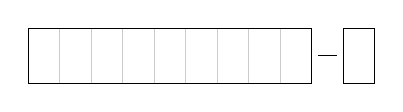
\begin{tikzpicture}[xscale=.4,yscale=.7]
    \draw[gray!40] ( 0, 0) grid      ( 9, 1);
    \draw          ( 0, 0) rectangle ( 9, 1);
    \draw          (10, 0) rectangle (11, 1);
    \draw (9 + .2, .5) -- (10 - .2, .5);
  \end{tikzpicture}%
}
\newcommand{\li}{\lstinline}
\providecommand{\pond}[1]{[{\small\textbf{#1\%}}]}

\lstdefinelanguage{py}{%
  classoffset=0,%
    morekeywords={%
      False,class,finally,is,return,None,continue,for,lambda,try,%
      True,def,from,nonlocal,while,and,del,global,not,with,print,%
      as,elif,if,or,yield,assert,else,import,pass,break,except,in,raise},%
    keywordstyle=\color{black!80}\bfseries,%
  classoffset=1,
    morekeywords={int,float,str,abs,len,raw_input,exit,range,min,max,%
      set,dict,tuple,list,bool,complex,round,sum,all,any,zip,map,filter,%
      sorted,reversed,dir,file,frozenset,open,%
      array,zeros,ones,arange,linspace,eye,diag,dot},
    keywordstyle=\color{black!50}\bfseries,%
  classoffset=0,%
  sensitive=true,%
  morecomment=[l]\#,%
  morestring=[b]',%
  morestring=[b]",%
  stringstyle=\em,%
}

\lstdefinelanguage{testcase}{%
  moredelim=[is][\bfseries]{`}{`},%
  backgroundcolor=\color{gray!20},%
}

\lstdefinelanguage{file}{%
  frame=single,%
}

\lstset{language=py}
\lstset{basicstyle=\ttfamily}
\lstset{columns=fixed}
\lstset{upquote=true}
\lstset{showstringspaces=false}
\lstset{rangeprefix=\#\ }
\lstset{includerangemarker=false}

\newlist{certamen}{enumerate}{1}
\setlist[certamen]{%
  label=\arabic*.,
  font=\LARGE\bfseries,%
  labelindent=-.5in,%
  leftmargin=0pt,%
  labelsep=1em%
}



\begin{document}

  \begin{enumerate}[font=\Large\bfseries]

    % Entender programas
    \item%[1a.]
      \pond{25}

      Indique qué es lo que imprimen los siguientes programas.

      \foreach \x in {1,2} {
        \noindent
        \begin{minipage}[b]{.5\textwidth}
          \lstinputlisting{p\x.py}
          \framebox[.8\textwidth]{\rule[10ex]{0pt}{0pt}}
          \vspace{0.4em}
        \end{minipage}
      }

    %\item[1b.]
      Rutee el siguiente programa
      e indique qué es lo que imprime.

      Cada vez que el valor de una variable cambie,
      ponga su valor en una nueva fila de la tabla.
      La tabla tiene filas de sobra.

      \begin{minipage}[T]{.5\textwidth}
        \lstinputlisting{ruteo.py}
        \framebox[.8\textwidth]{\rule[10ex]{0pt}{0pt}}
      \end{minipage}
      \begin{minipage}[t]{.4\textwidth}\centering
        \begin{tabular}{|p{4em}|p{4em}|p{4em}|}\hline
            \cc{j} & \cc{c} & \cc{p} \\ \hline\hline
            && \\\hline && \\\hline && \\\hline && \\\hline && \\\hline
            && \\\hline && \\\hline && \\\hline && \\\hline && \\\hline
            && \\\hline && \\\hline && \\\hline && \\\hline && \\\hline
            && \\\hline && \\\hline && \\\hline && \\\hline && \\\hline
            && \\\hline && \\\hline && \\\hline && \\\hline && \\\hline
         \end{tabular}
      \end{minipage}

    \newpage
    \item%[2.]
      \pond{25}
      Un tablero de ajedrez es una grilla
      de ocho filas y ocho columnas, numeradas de 1 a 8.
      Dos de las piezas del juego de ajedrez son el alfil y la torre.
      El alfil se desplaza en diagonal,
      mientras que la torre se desplaza horizontal o verticalmente.
      Una pieza puede ser capturada por otra
      si está en una casilla a la cual la otra puede desplazarse:

      \tikzstyle{pieza}=[circle, inner sep=1pt]
      \tikzstyle{ma}=[ultra thick, densely dotted, black!45]
      \tikzstyle{mt}=[ultra thick, dashed, black!45]
      \def\tablero{%
        \foreach\row in {2,4,...,8}
          \foreach\col in {1,3,...,7}
            \fill[black!20] (\row - .5, \col - .5) rectangle (\row + .5, \col + .5);
        \foreach\row in {1,3,...,7}
          \foreach\col in {2,4,...,8}
            \fill[black!20] (\row - .5, \col - .5) rectangle (\row + .5, \col + .5);
        \draw (.4, .4) rectangle (8.6, 8.6);
        \foreach\row in {1,...,8}
          \node[anchor=east]  at (.4, \row) {\footnotesize\row};
        \foreach\col in {1,...,8}
          \node[anchor=south] at (\col, .4) {\footnotesize\col};
      }
      \begin{tikzpicture}[scale=.5, yscale=-1]
        \tablero
        \node[pieza] (alfil) at (6, 7) {A};
        \node[pieza] (torre) at (3, 4) {T};
        \draw[ma] (1 - .3, 2 - .3) -- (alfil);
        \draw[ma] (5 - .3, 8 + .3) -- (alfil);
        \draw[ma] (8 + .3, 5 - .3) -- (alfil);
        \draw[ma] (7 + .3, 8 + .3) -- (alfil);
        \draw[mt] (3     , 1 - .3) -- (torre);
        \draw[mt] (3     , 8 + .3) -- (torre);
        \draw[mt] (1 - .3, 4     ) -- (torre);
        \draw[mt] (8 + .3, 4     ) -- (torre);
        \node at (4.5, 9.3) {\footnotesize Alfil captura a torre};
      \end{tikzpicture}
      \hfil
      \begin{tikzpicture}[scale=.5, yscale=-1]
        \tablero
        \node[pieza] (alfil) at (4, 3) {A};
        \node[pieza] (torre) at (4, 7) {T};
        \draw[ma] (2 - .3, 1 - .3) -- (alfil);
        \draw[ma] (1 - .3, 6 + .3) -- (alfil);
        \draw[ma] (6 + .3, 1 - .3) -- (alfil);
        \draw[ma] (8 + .3, 7 + .3) -- (alfil);
        \draw[mt] (4     , 1 - .3) -- (torre);
        \draw[mt] (4     , 8 + .3) -- (torre);
        \draw[mt] (1 - .3, 7     ) -- (torre);
        \draw[mt] (8 + .3, 7     ) -- (torre);
        \node at (4.5, 9.3) {\footnotesize Torre captura a alfil};
      \end{tikzpicture}
      \hfil
      \begin{tikzpicture}[scale=.5, yscale=-1]
        \tablero
        \node[pieza] (alfil) at (3, 3) {A};
        \node[pieza] (torre) at (5, 8) {T};
        \draw[ma] (1 - .3, 1 - .3) -- (alfil);
        \draw[ma] (1 - .3, 5 + .3) -- (alfil);
        \draw[ma] (5 + .3, 1 - .3) -- (alfil);
        \draw[ma] (8 + .3, 8 + .3) -- (alfil);
        \draw[mt] (5     , 1 - .3) -- (torre);
        %\draw[mt] (5     , 8 + .3) -- (torre);
        \draw[mt] (8 + .3, 8     ) -- (torre);
        \draw[mt] (1 - .3, 8     ) -- (torre);
        \node at (4.5, 9.3) {\footnotesize Ninguna pieza captura};
      \end{tikzpicture}

      Escriba un programa que reciba como entrada
      las posiciones en el tablero de un alfil y de una torre,
      e indique cuál pieza captura a la otra:

      \begin{minipage}[t]{.28\textwidth}
        \lstinputlisting[language=testcase,frame=single]{caso2a.txt}
      \end{minipage}
      \hfil
      \begin{minipage}[t]{.28\textwidth}
        \lstinputlisting[language=testcase,frame=single]{caso2b.txt}
      \end{minipage}
      \hfil
      \begin{minipage}[t]{.28\textwidth}
        \lstinputlisting[language=testcase,frame=single]{caso2c.txt}
      \end{minipage}

      Suponga que todos los datos ingresados son válidos.
      Su programa debe funcionar para tableros de \(1000\times 1000\).

    % Programas simples (entrada, asignaciones, salida)
    \newpage
    \item%[3.]
      \pond{25}
      En estadística descriptiva,
      se define el \emph{rango} de un conjunto de datos reales
      como la diferencia entre el mayor y el menor de los datos.

      Por ejemplo, si los datos son:
      \(
        \begin{bmatrix}
        5.96 & 6.74 & 7.43 & 4.99 & 7.20 & 0.56 & 2.80 
        \end{bmatrix}
      \)
      entonces el rango es \(7.43 - 0.56 = 6.87\).

      \begin{minipage}[t]{.43\textwidth}
        Escriba un programa que:
        \begin{itemize}
          \item pregunte al usuario cuántos datos serán ingresados,
          \item pida al usuario ingresar los datos uno por uno, y
          \item entregue como resultado el rango de los datos.
        \end{itemize}
        Suponga que todos los datos ingresados son válidos.
      \end{minipage}
      \hfill
      \begin{minipage}[t]{.45\textwidth}
        \lstinputlisting[language=testcase,frame=single]{caso3.txt}
      \end{minipage}

    % Algoritmos sencillos
    \newpage
    \item%[4.]
      \pond{25}
      En finanzas,
      el \emph{valor actual neto} es un indicador
      de cuán rentable será un proyecto.

      Se calcula sumando
      los flujos de dinero de cada mes
      divididos por \((1 + r)^n\),
      donde \(n\) es el número del mes
      y \(r\) es la tasa de descuento mensual,
      y restando la inversión inicial.

      Por ejemplo,
      en un proyecto en que la inversión inicial es \(\$900\),
      los flujos de dinero estimados para los primeros cuatro meses son
      \(\$550\), \(\$230\), \(\$341\) y \(\$190\),
      y la tasa de descuento mensual es de 4\%,
      el valor actual neto es:
      \[
        \text{VAN} = -900 +
                     \frac{550}{(1 + 0.04)^1} +
                     \frac{230}{(1 + 0.04)^2} +
                     \frac{341}{(1 + 0.04)^3} +
                     \frac{190}{(1 + 0.04)^4}.
      \]

      Si el VAN da negativo, entonces no es conveniente comenzar el proyecto.

      \begin{minipage}[t]{.43\textwidth}
        Escriba un programa que pida al usuario ingresar la inversión inicial
        y el porcentaje de tasa de descuento.
        A continuación,
        debe preguntar el flujo de dinero estimado para cada mes
        y mostrar cuál es la parte entera del VAN hasta ese momento.

        El programa debe terminar apenas el VAN comience a dar positivo.

        \vspace{1ex}
        Suponga que todos los datos ingresados son válidos.
      \end{minipage}
      \hfill
      \begin{minipage}[t]{.45\textwidth}
        \lstinputlisting[language=testcase,frame=single]{caso4.txt}
      \end{minipage}


    % Problema de aplicación
    %\newpage
    %\item

    %  Las \emph{ecuaciones de Lotka-Volterra}
    %  describen cómo cambian las poblaciones de dos especies en un ecosistema,
    %  en el que una de ellas es depredadora de la otra.

    %  En un día dado,
    %  \(x\) representa el número de depredadores, e
    %  \(y\) el número de presas.
    %  La variación de ambas cantidades durante el día
    %  es aproximadamente:
    %  \begin{align*}
    %    \Delta x &\approx \phantom{-}x(\alpha - \beta  y),\\
    %    \Delta y &\approx           -y(\gamma - \delta x),
    %  \end{align*}
    %  donde \(\alpha\), \(\beta\), \(\gamma\) y \(\delta\)
    %  son parámetros que dependen de las características del ecosistema.

    %  Por lo tanto, después de cada día,
    %  las nuevas poblaciones son \(x + \Delta x\) e \(y + \Delta y\).

    %  Suponga que la dinámica de un ecosistema
    %  compuesto por lobos y conejos
    %  está descrita por los parámetros:
    %  \(\alpha = 0.003\),
    %  \(\beta  = 0.4\),
    %  \(\gamma = 0.005\) y
    %  \(\delta = 0.6\).

    %  Escriba un programa para determinar
    %  si los conejos se extinguen en menos de 100 días.
    %  El programa debe recibir como entrada
    %  las poblaciones iniciales de lobos y conejos.

    %  Si los conejos se extinguen en menos de 100 días,
    %  la salida debe mostrar en cuántos días ocurre esto.

    %  Si los conejos no se extinguen,
    %  la salida debe decir cuál es la población de conejos
    %  en el centésimo día.

  \end{enumerate}
\end{document}

